% This is the Reed College LaTeX thesis template. Most of the work
% for the document class was done by Sam Noble (SN), as well as this
% template. Later comments etc. by Ben Salzberg (BTS). Additional
% restructuring and APA support by Jess Youngberg (JY).
% Your comments and suggestions are more than welcome; please email
% them to cus@reed.edu
%
% See https://www.reed.edu/cis/help/LaTeX/index.html for help. There are a
% great bunch of help pages there, with notes on
% getting started, bibtex, etc. Go there and read it if you're not
% already familiar with LaTeX.
%
% Any line that starts with a percent symbol is a comment.
% They won't show up in the document, and are useful for notes
% to yourself and explaining commands.
% Commenting also removes a line from the document;
% very handy for troubleshooting problems. -BTS

% As far as I know, this follows the requirements laid out in
% the 2002-2003 Senior Handbook. Ask a librarian to check the
% document before binding. -SN

%%
%% Preamble
%%
% \documentclass{<something>} must begin each LaTeX document
\documentclass[12pt,twoside]{reedthesis}
% Packages are extensions to the basic LaTeX functions. Whatever you
% want to typeset, there is probably a package out there for it.
% Chemistry (chemtex), screenplays, you name it.
% Check out CTAN to see: https://www.ctan.org/
%%
\usepackage{graphicx,latexsym}
\usepackage{amsmath}
\usepackage{amssymb,amsthm}
\usepackage{longtable,booktabs,setspace}
\usepackage{chemarr}%% Useful for one reaction arrow, useless if you're not a chem major
\usepackage[hyphens]{url}
% Added by CII
\usepackage{hyperref}
\usepackage{lmodern}
\usepackage{float}
\floatplacement{figure}{H}
% Thanks, @Xyv
\usepackage{calc}
% End of CII addition
\usepackage{rotating}


% Next line commented out by CII
%%% \usepackage{natbib}
% Comment out the natbib line above and uncomment the following two lines to use the new
% biblatex-chicago style, for Chicago A. Also make some changes at the end where the
% bibliography is included.
%\usepackage{biblatex-chicago}
%\bibliography{thesis}


% Added by CII (Thanks, Hadley!)
% Use ref for internal links
\renewcommand{\hyperref}[2][???]{\autoref{#1}}
\def\chapterautorefname{Chapter}
\def\sectionautorefname{Section}
\def\subsectionautorefname{Subsection}
% End of CII addition

% Added by CII
\usepackage{caption}
\captionsetup{width=5in}
% End of CII addition



% \usepackage{times} % other fonts are available like times, bookman, charter, palatino

% Syntax highlighting #22

% To pass between YAML and LaTeX the dollar signs are added by CII
\title{Bayesian Hierarchial Modeling of Historical Irrigaiton Patterns}
\author{Rachel Ledig}
% The month and year that you submit your FINAL draft TO THE LIBRARY (May or December)
\date{July 2021}
\division{Albrecht Daniel Thaer Institute for Agricultural and Horticultural Sciences}
\advisor{Dr.~Tobias Krueger}
\institution{University of Humboldt}
\degree{Master of Science}
\bday{Nov 17, 1991}
\bplace{California, USA}
\matriculation{602220}
\email{\href{mailto:ledigrac@hu-berlin.de}{\nolinkurl{ledigrac@hu-berlin.de}}}
%If you have two advisors for some reason, you can use the following
% Uncommented out by CII
\altadvisor{Dr.~Christian Schleyer}
\supervisor{Dr.~Fabian Stenzel}
% End of CII addition

%%% Remember to use the correct department!
\department{Faculty of Life Sciences}
% if you're writing a thesis in an interdisciplinary major,
% uncomment the line below and change the text as appropriate.
% check the Senior Handbook if unsure.
%\thedivisionof{The Established Interdisciplinary Committee for}
% if you want the approval page to say "Approved for the Committee",
% uncomment the next line
%\approvedforthe{Committee}

% Added by CII
%%% Copied from knitr
%% maxwidth is the original width if it's less than linewidth
%% otherwise use linewidth (to make sure the graphics do not exceed the margin)
\makeatletter
\def\maxwidth{ %
  \ifdim\Gin@nat@width>\linewidth
    \linewidth
  \else
    \Gin@nat@width
  \fi
}
\makeatother

% From {rticles}
\newlength{\csllabelwidth}
\setlength{\csllabelwidth}{3em}
\newlength{\cslhangindent}
\setlength{\cslhangindent}{1.5em}
% for Pandoc 2.8 to 2.10.1
\newenvironment{cslreferences}%
  {}%
  {\par}
% For Pandoc 2.11+
% As noted by @mirh [2] is needed instead of [3] for 2.12
\newenvironment{CSLReferences}[2] % #1 hanging-ident, #2 entry spacing
 {% don't indent paragraphs
  \setlength{\parindent}{0pt}
  % turn on hanging indent if param 1 is 1
  \ifodd #1 \everypar{\setlength{\hangindent}{\cslhangindent}}\ignorespaces\fi
  % set entry spacing
  \ifnum #2 > 0
  \setlength{\parskip}{#2\baselineskip}
  \fi
 }%
 {}
\usepackage{calc} % for calculating minipage widths
\newcommand{\CSLBlock}[1]{#1\hfill\break}
\newcommand{\CSLLeftMargin}[1]{\parbox[t]{\csllabelwidth}{#1}}
\newcommand{\CSLRightInline}[1]{\parbox[t]{\linewidth - \csllabelwidth}{#1}}
\newcommand{\CSLIndent}[1]{\hspace{\cslhangindent}#1}

\renewcommand{\contentsname}{Table of Contents}
% End of CII addition

\setlength{\parskip}{0pt}

% Added by CII

\providecommand{\tightlist}{%
  \setlength{\itemsep}{0pt}\setlength{\parskip}{0pt}}

\Acknowledgements{
Adjust your expectations accordingly (\protect\hyperlink{ref-teamStanReferenceManual}{Team n.d.})
}

\Dedication{
To Mom, Dad, Sis, and Fi.
}

\Preface{

}

\Abstract{
The preface pretty much says it all.

\par

Second paragraph of abstract starts here.
}

\Abbreviations{
\begin{tabular}{rp{0.2cm}lp{1cm}rp{0.2cm}l} IF & &  Irrigaion Fraction \\ BS  & &  Bisulfite \\ SDS  & &  Sodium dodecyl sulfate  \\ TMT  & & Tandem mass tags \\ \end{tabular}
}

	\usepackage{wrapfig}
	\usepackage{booktabs}
 \usepackage{longtable}
 \usepackage{array}
 \usepackage{multirow}
 \usepackage{wrapfig}
 \usepackage{float}
 \usepackage{colortbl}
 \usepackage{pdflscape}
 \usepackage{tabu}
 \usepackage{threeparttable}
 \usepackage{threeparttablex}
 \usepackage[normalem]{ulem}
 \usepackage{makecell}
 \usepackage{xcolor}
% End of CII addition
%%
%% End Preamble
%%
%
\begin{document}

% Everything below added by CII
  \maketitle

\frontmatter % this stuff will be roman-numbered
\pagestyle{empty} % this removes page numbers from the frontmatter
  \begin{acknowledgements}
    Adjust your expectations accordingly (\protect\hyperlink{ref-teamStanReferenceManual}{Team n.d.})
  \end{acknowledgements}

  \hypersetup{linkcolor=black}
  \setcounter{secnumdepth}{2}
  \setcounter{tocdepth}{2}
  \tableofcontents


  \listoftables

  \listoffigures
  \begin{abbreviations}
    \begin{tabular}{rp{0.2cm}lp{1cm}rp{0.2cm}l} IF & &  Irrigaion Fraction \\ BS  & &  Bisulfite \\ SDS  & &  Sodium dodecyl sulfate  \\ TMT  & & Tandem mass tags \\ \end{tabular}
  \end{abbreviations}
  \begin{abstract}
    The preface pretty much says it all.

    \par

    Second paragraph of abstract starts here.
  \end{abstract}
  \begin{dedication}
    To Mom, Dad, Sis, and Fi.
  \end{dedication}
\mainmatter % here the regular arabic numbering starts
\pagestyle{fancyplain} % turns page numbering back on

\hypertarget{intro}{%
\chapter{Introduction}\label{intro}}

The practice of irrigation, and its subsequent impacts, have far reaching effects for the global economy, food and water supply, and environment. Irrigated land accounts for 20\% of the global cultivated land area which derives 40\% of the global food supply \protect\hyperlink{ref-portmannMIRCA2000GlobalMonthly2010a}{Portmann, Siebert, and Döll} (\protect\hyperlink{ref-portmannMIRCA2000GlobalMonthly2010a}{2010}), 70\% of water withdrawls from ground water aquifers are used for irrigation (\protect\hyperlink{ref-faoStateWorldLand2011}{FAO 2011}), and

\hypertarget{objectives}{%
\section{Objectives}\label{objectives}}

Ultimately, the agricultural system will continue to demand more water while competing with other sectors over decreasing water availability in the coming years. With this pressure, farmers will aim to be as efficient as possible by increasing their yields which, in certain areas and under certain conditions, can be done by irrigating their fields. Understanding where, when, and why farmers decide to begin irrigating is important to understand water demands now and in the future. Unfortunately, irrigation expansion is seldom studied, with few studies using statistical modeling techniques to investigate the role that biophysical, economic, and political factors play in the spread of irrigation infrastructure in the present. None do so historically. This leads to the first and overarching research question:

\emph{Which factors (drivers) have influenced the expansion of irrigation in both time and space over the past 100 years?}

By understanding under which conditions irrigation infrastructure is built could be coupled with projections of future climate and economic scenarios, allowing us to get a better idea of scales of agricultural production, land use, and water needs in the coming years. In order to eventually extrapolate to the future, predictive accuracy needs to be addressed. This can be done by separating data into training and testing datasets, model tuning, and error estimation.

Several other questions smaller questions arise in regard to drivers of expansion which are interesting to investigate. Such as:
\begin{itemize}
\item
  Which has a larger influence on irrigation expansion patterns, biophysical or socio-economic factors?
\item
  Do rates of irrigation expansion differ depending on crop type?
\end{itemize}
Both of these questions have interesting policy implications, should large trends be present in the model and analysis.

The time series component of this data set also gives rise to some interesting questions.
\begin{itemize}
\item
  Expansion rates of total irrigated area differ temporally, what could be the drivers for this difference?
\item
  Is there a temporal delay in irrigation expansion based on the influence of certain drivers, and if so how much?
\end{itemize}


\hypertarget{Theory}{%
\chapter{Theoretical Basis}\label{Theory}}

This chapter details the theoretical basis for this thesis. Initially, literature will be reviewed beginning with irrigation expansion drivers in Section \ref{drivers} and followed by a detailed account of prior irrigation modeling studies in Section \ref{irrmodslit}. Finally, an account of the basics of Bayesian inference will be described in Section \ref{bayesintro}.

\hypertarget{lit}{%
\section{Literature}\label{lit}}

Foundations for the model proposed in this thesis begin at the literature level. In order to appropriately select predictors for the proposed model, it is necessary to look at what drives irrigation from multiple angles including studies on farmer preferences, policy decisions, manuals, reports, and other modeling studies.

\hypertarget{drivers}{%
\subsection{Drivers of Irrigation Expansion}\label{drivers}}

Understanding the mechanisms behind irrigation and the features of irrigation systems is imperative to understanding why, when, and where irrigation is implemented. According to the \protect\hyperlink{ref-faoGuidelinesDesigningEvaluating1989}{FAO and Walker} (\protect\hyperlink{ref-faoGuidelinesDesigningEvaluating1989}{1989}), the choice by the farmer of irrigation technology is dependent on several intertwined socio-economic and biophysical concerns. Multitudes of literature exist detailing the considerations necessary when choosing an irrigation system, but little exists on why farmers choose to irrigate in the first place. Although the distinction is notable and directly equating the choice of a specific irrigation technology to the decision to begin irrigating is perhaps naive, it is important to understand that the decision to irrigate \emph{is not possible} without the simultaneous choice of an irrigation technology. Therefore using the irrigation technology selection criteria outlined by \protect\hyperlink{ref-faoGuidelinesDesigningEvaluating1989}{FAO and Walker} (\protect\hyperlink{ref-faoGuidelinesDesigningEvaluating1989}{1989}) as a basis to discuss drivers of irrigation expansion is justified.

By using these areas as a guideline for what farmers are concerned about when establishing an irrigation system and why those concerns exist, not only can the causal relationship between external conditions and irrigation expansion be investigated, but appropriate predictors for the hierarchical model can also be selected. These eight components are detailed in the subsections below.

To begin, it is important to know a little bit about irrigation systems. Irrigation systems can be divided into two main systems: gravity fed which includes all types of surface irrigation, and mechanized pump systems, such as sprinkler or localized distributions (\protect\hyperlink{ref-bjornebergIRRIGATIONMethods2013}{Bjorneberg 2013}). Surface irrigation, such as furrow, basin, or border irrigation, is the oldest, simplest, and cheapest method available and used on around 85\% of the irrigated land in the world (\protect\hyperlink{ref-bjornebergIRRIGATIONMethods2013}{Bjorneberg 2013}; \protect\hyperlink{ref-holzapfelIrrigationAgriculture2008}{Holzapfel and Mariño 2008}). Pumped irrigation systems are less common globally. Different types of irrigation can be seen in Figure \ref{fig:irrigationtypes}.
\begin{figure}

{\centering 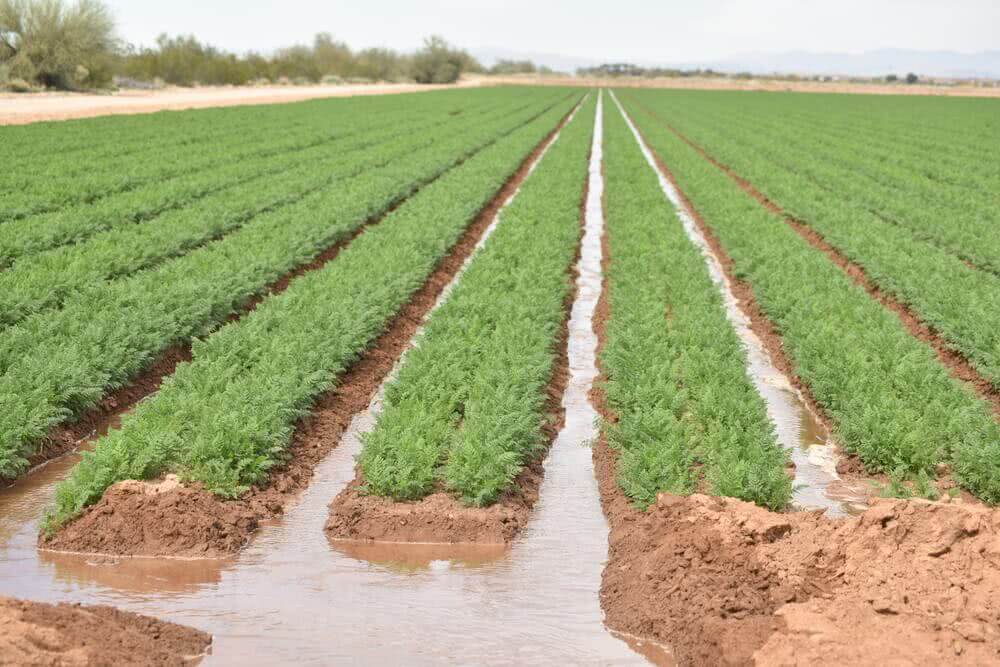
\includegraphics[width=0.3\linewidth,height=0.2\textheight]{figure/FurrowPic} 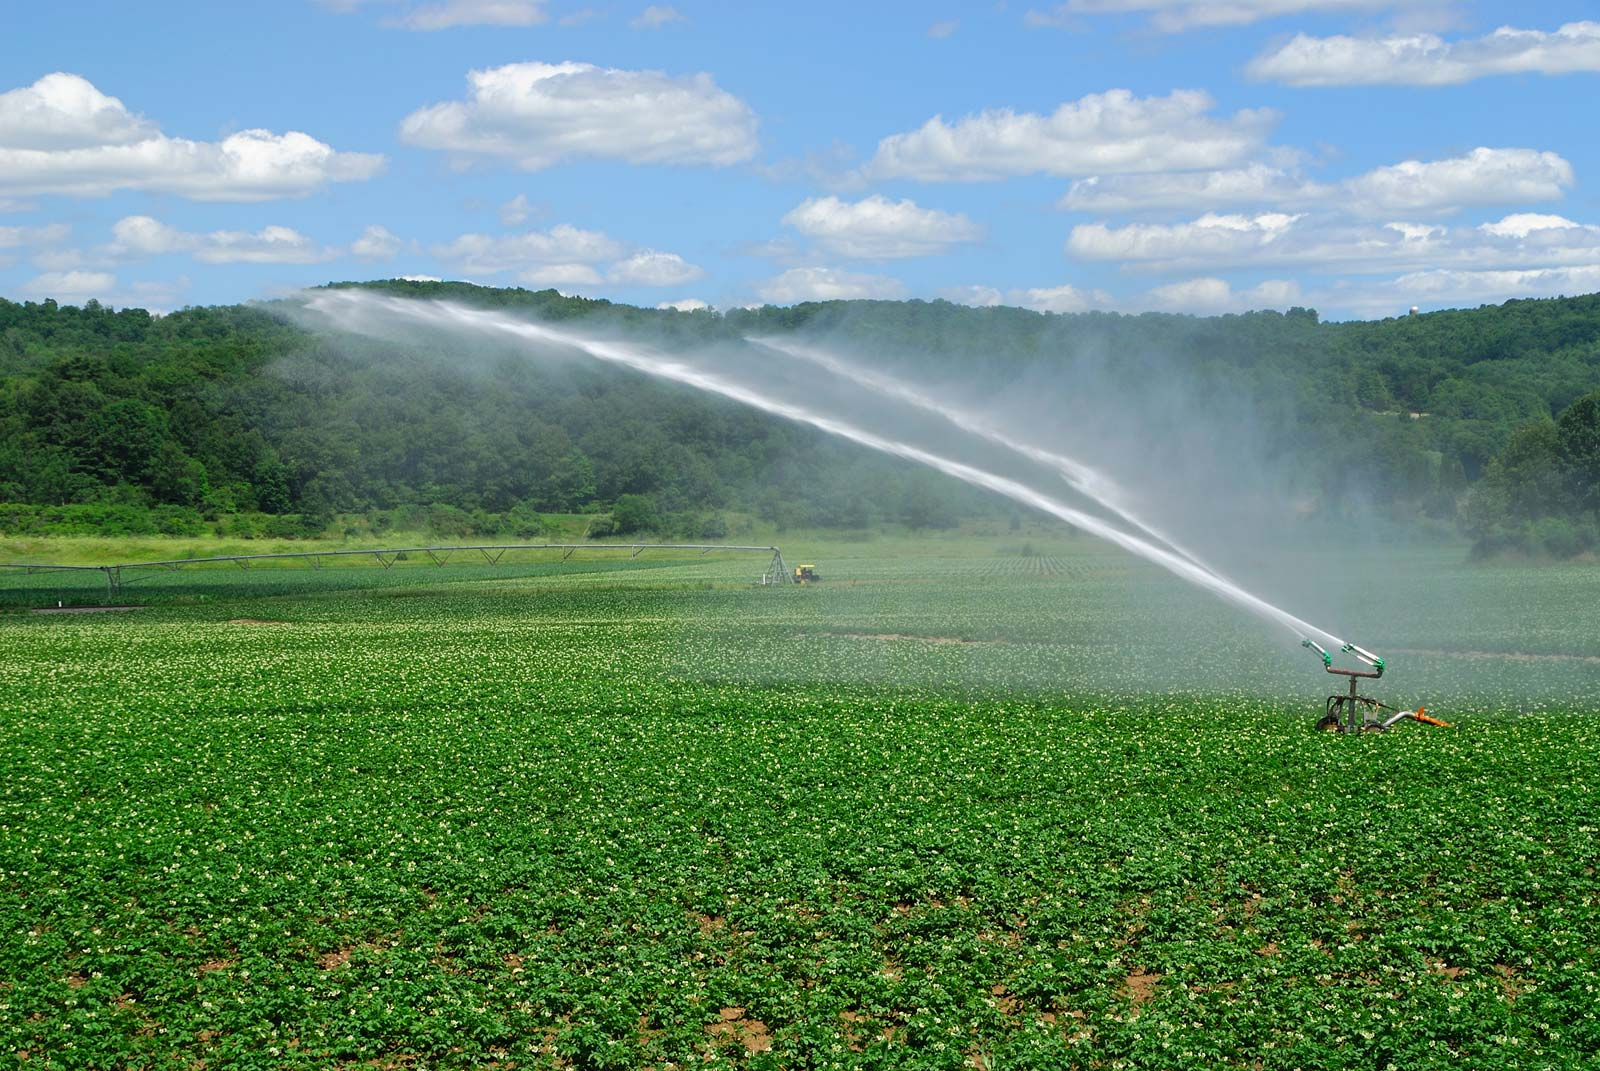
\includegraphics[width=0.3\linewidth,height=0.2\textheight]{figure/Irrigation-sprinklers} 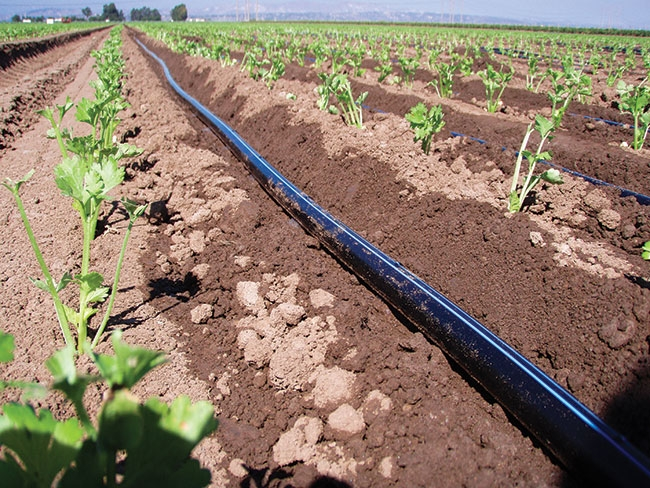
\includegraphics[width=0.3\linewidth,height=0.2\textheight]{figure/DripIrrigation} 

}

\caption{Furrow, Sprinkler and Drip irrigation  [@GoogleImages2021]}\label{fig:irrigationtypes}
\end{figure}
\hypertarget{water}{%
\subsubsection{Water}\label{water}}

Water supply is a core component of irrigation and can be divided into two main dimensions, water quantity, and water quality. As water quality matters more for the choice of a specify irrigation technology, it will not be discussed in detail below. Water quantity, however, is a large concern when deciding if a farmer can irrigate. In the natural world, water comes from three sources: rain, surface water (rivers, lakes, reservoirs, etc.), or groundwater (aquifers).

Precipitation, specifically rainfall, is not technically an irrigation water source as is applied directly to crops without any irrigation system. As a result, rainfall, a free source of crop water, currently sustains roughly 80\% of the global cultivated area which produces 60\% of the total crop production (\protect\hyperlink{ref-worldwaterassesnentprogramUnitedNationsWorld2009}{Program and UNESCO 2009}). Although direct rainfall is the predominant method for watering crops and can nullify the need for any irrigation technology, meeting crop water demand with rainfall can be difficult as rainfall can be extremely varied in both space and time. Spatially, different regions receive different annual amounts of rainfall, with tropical and temperate zones receiving more rainfall than semi-arid or arid regions (\protect\hyperlink{ref-forsethTerrestrialBiomes2010}{Forseth 2010}). However, mean annual rainfall does not show the whole picture, and when deciding whether the amount of precipitation in a region is sufficient to sustain crop growth, it is important to remember that rainfall can heavily vary in seasonality, as well. Wet and dry seasons dictate the boom and bust of vegetation in some tropical and sub-tropical regions {[}CITATION{]}. The coincidence of rainfall and crop growing season is integral for farmers as crop water demands must be met during the specific periods of the crop's growing cycle. One benefit of rain-fed agriculture is that rainwater is naturally of high quality, meaning that it is free of solids and harmful substances that other water sources may have (\protect\hyperlink{ref-douglascox2015}{Douglas Cox et al. 2015}). Although, it should be noted that patterns of rainfall are shifting with the effects of climate change. When long-standing climactic patterns change, differences in annual rainfall amounts, duration of the wet and dry seasons, and intensity of rainfall have consequences for both farmers and crops, making planning for a productive growing season more difficult in some areas (\protect\hyperlink{ref-rockstromManagingWaterRainfed2010}{Rockström et al. 2010}). These changes have the potential to incentivize the shift from rainfed agriculture to irrigated.

Surface water is only applied to crops through an irrigation system, unlike rainwater. Surface water is water that is collected, from precipitation, runoff, and up-welling of groundwater resources, on the surface of the planet (in rivers, lakes, ponds, and dams). Surface water is the most common water source for irrigation as its supply is generally less variable than precipitation and easier to access than groundwater. As a result, 54\% of the area available for irrigation is irrigated with surface water (\protect\hyperlink{ref-siebertGroundwaterUseIrrigation2010}{Siebert et al. 2010}; \protect\hyperlink{ref-thenkabailGlobalIrrigatedArea2009}{Thenkabail et al. 2009}). Surface water, due to the fact that it is accumulative, potentially passes through many environments before it is extracted by the farmer and applied to the field, meaning that issues with water quality are more common. Pollution, sediment, and salts must be monitored to ensure that the surface water can be applied to crops and is able to pass through the specific irrigation distribution system (\protect\hyperlink{ref-faoIrrigationManualPlanning2001}{FAO and SAFR 2001}). Again, it should be pointed out that since the original source of most surface water is precipitation in some form, it is also susceptible to changes in precipitation patterns due to climate change.

Groundwater, water that is stored below ground in aquifers, is a collection of water that has infiltrated through the soil over many years. As a source of clean reliable irrigation water, groundwater is unparalleled (\protect\hyperlink{ref-siebertGroundwaterUseIrrigation2010}{Siebert et al. 2010}). The water stored in aquifers is of high quality and much more resistant to seasonal changes in precipitation than surface water. Groundwater's largest issue, with respect to its use as a source of water for irrigation, is access. Multiple methods for groundwater extraction exist but most are more costly than surface water withdrawals. However, in semi-arid or arid regions where surface water may also be seasonal or non-existent, extraction of groundwater for irrigation becomes more economically viable as its use can sustain large populations (E.g. regions in the middle east).

Ultimately, rainfall is always the default source for farmers to supply water to their crops, and only when rainfall is not sufficient during necessary parts of the crop growing season, do farmers consider using irrigation to meet the crop water demand.

\hypertarget{topo}{%
\subsubsection{Topography}\label{topo}}
\begin{figure}
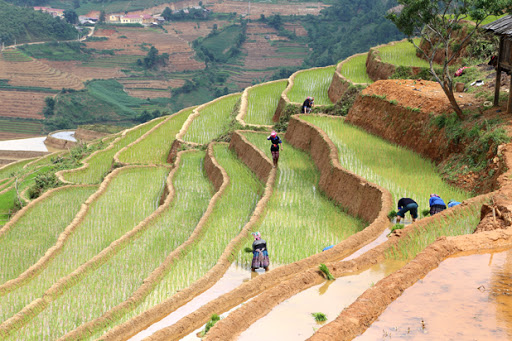
\includegraphics[width=0.5\linewidth]{figure/TerraceRicePic} \caption{Terraced rice in Vietnam [@GoogleImages2021]}\label{fig:unnamed-chunk-4}
\end{figure}
Steep topography can prevent the implementation of the majority of most common and basic surface irrigation systems, such as furrow (using long channels to water crops) or basin (flooding of field sections) irrigation. Generally, for this type of irrigation to be used field slopes need to have less than a 5\% incline, which limits the application of this simple type of irrigation to valleys and flatlands (\protect\hyperlink{ref-faoIrrigationManualPlanning2001}{FAO and SAFR 2001}).

Other types of irrigation, sprinkler or localized systems, can be utilized in steeper environments, but are often more costly than simple surface irrigation techniques. There are some ingenious examples of farmers working with topography to use simple irrigation methods and adapt to steeper slopes: rice terraces in South East Asia use basin irrigation to cultivate paddy rice on extremely steep slopes (\protect\hyperlink{ref-adachiAgriculturalTechnologiesTerraced2007}{Adachi 2007}). However, in general, steep slopes are rarely irrigated with surface irrigation methods.

\hypertarget{soil}{%
\subsubsection{Soil}\label{soil}}

Soil composition, in the context of irrigation, is important because different soils have different capacities to store and infiltrate water, meaning that different types of irrigation systems may be necessary to ensure that crops are able to get the water that they need (\protect\hyperlink{ref-faoGuidelinesDesigningEvaluating1989}{FAO and Walker 1989}). For example, sandy soils retain less water and drain faster, meaning that they must be irrigated more frequently but with less water. In this case, surface irrigation methods that apply large amounts of water to a field at one time may be less suited for these soils (\protect\hyperlink{ref-faoIrrigationWaterManagement1986a}{FAO, Brouwer, and Heibloem 1986}). In addition, as the soil type dictates the infiltration rate of irrigation water and therefore the rate of application, the soil type combined with the specific irrigation method chosen may impose requirements on the consistency and volume of the water supply. For the context of this thesis, soil composition will be largely ignored as the oftentimes soil composition limits the type of irrigation used, not the absence or presence of it. However, it is important to note that as surface irrigation methods, which are more common worldwide, are less suitable for certain soil types (E.g. sandy soils), there may be circumstances in which given a specific soil type, irrigation would be inefficient.

\hypertarget{crops}{%
\subsubsection{Crops}\label{crops}}

Crop type also has the potential to influence the presence/absence of irrigation and the type used as different crops require different amounts of water over the the growing period (\protect\hyperlink{ref-faoIrrigationWaterManagement1986}{FAO et al. 1986}). Staple crops that need to be irrigated are rarely irrigated with sprinkler or localized (drip) systems as these systems are much more costly than surface irrigation. Sprinkler and localized systems are almost always reserved for fruits and vegetables, so-called cash crops (\protect\hyperlink{ref-faoIrrigationWaterManagement1985}{FAO et al. 1985}).

\hypertarget{combatibility}{%
\subsubsection{Compatibility}\label{combatibility}}

Irrigation technologies must be a benefit not a burden to the farmer and the choice to irrigate must fit within the given growing and harvesting needs of a particular crop. Irrigation must not impede the usage of pruning or harvesting machinery (\protect\hyperlink{ref-faoGuidelinesDesigningEvaluating1989}{FAO and Walker 1989}). In addition, the farmers must be able to work with the chosen irrigation technology. Sprinkler and localized systems are more complicated than surface irrigation, however, surface irrigation requires more manual input from the farmer. Surface irrigation is also easier to maintain than other types of irrigation (\protect\hyperlink{ref-faoIrrigationWaterManagement1986a}{FAO, Brouwer, and Heibloem 1986}). This is less of a concern for this thesis, as compatibility issues between crop type, irrigation system, farmer knowledge, and other farm machinery is not the main focus.

\hypertarget{econ}{%
\subsubsection{Economics}\label{econ}}

The economics of specific irrigation systems and the choice to irrigate is important for farmers, as even the simplest surface irrigation methods are not without costs. Water, energy, materials, labor, maintenance, and monitoring costs must all be considered when deciding to begin irrigating and which irrigation system to choose (\protect\hyperlink{ref-faoGuidelinesDesigningEvaluating1989}{FAO and Walker 1989}). According to \protect\hyperlink{ref-faoIrrigationManualPlanning2001}{FAO and SAFR} (\protect\hyperlink{ref-faoIrrigationManualPlanning2001}{2001}), for small farms in Sub-Saharan Africa, up to 80\% of the costs to develop an irrigation system stems from water resource procurement, such as construction of a dam. In addition, the authors note that the cost for cubic meter of water is increasing in this region as well, putting more economic pressure on the farmers.

\hypertarget{socinf}{%
\subsubsection{Social Influences}\label{socinf}}

However, there are ways to shift the costs of establishing irrigation from the individual farmer to the collective. Grass-roots, bottom-up irrigation cooperatives or schemes may be set up to share the construction, maintenance, and monitoring of shared irrigation and water transportation infrastructure (\protect\hyperlink{ref-faoGuidelinesDesigningEvaluating1989}{FAO and Walker 1989}). \protect\hyperlink{ref-faoGuidelinesDesigningEvaluating1989}{FAO and Walker} (\protect\hyperlink{ref-faoGuidelinesDesigningEvaluating1989}{1989}) note that there are often several levels involved in the organization of irrigation schemes. These include the individual farmers who participate at the field level; the local farmers' collectives who manage operation, maintenance, allocation, and conflicts; the governing body at the local or state level that deals with water distribution and funding. Each actor has different needs, power, and roles ensuring the management of local irrigation. Examples of irrigation schemes are common globally and historically.

\hypertarget{extinf}{%
\subsubsection{External Influences}\label{extinf}}

Sometimes external factors play a large role in stimulating irrigation expansion. Social trends, governmental programs, and conflicts among others can influence the rate of irrigation expansion at a sub-national, national, or regional level. This type of expansion could be labeled as top-down, as generally there are larger actors pushing or incentivising the construction of irrigation infrastructure, in comparison to the bottom-up dynamic of locally organized irrigation schemes.

\protect\hyperlink{ref-angelakisIrrigationWorldAgricultural2020}{Angelakis et al.} (\protect\hyperlink{ref-angelakisIrrigationWorldAgricultural2020}{2020}) details explicitly some of these trends that have occurred during the last century. In Spain, during the reign of Francisco Franco,\footnote{0.083° Longitude by 0.083° Latitude, or at the equator, a 9.3km by 9.3km grid cell} the government began a national water development plan to settle small farmers. This campaign created the foundation for Spain's expansive irrigated agricultural system today, the largest irrigated area in the European Union. Another instance that \protect\hyperlink{ref-angelakisIrrigationWorldAgricultural2020}{Angelakis et al.} (\protect\hyperlink{ref-angelakisIrrigationWorldAgricultural2020}{2020}) discusses is the sudden overall increase in irrigated area after the Second World War, which is attributed to two aspects: a sudden population increase and developments in technology. The population increase, due to increased birthrates and an extension of life span due to medical advances, created a demand for more food and advances in technology, specifically those that were necessary to optimize pumps needed for pressurized irrigation and water transportation systems. Both of these changes resulted in a rapid global expansion of irrigated area. Other examples exist such as the Green Revolution, or Third Agricultural Revolution,\footnote{The act of harvesting rainwater during rain and then later applying it to crops.} also spurred trends of irrigation expansion, particularly in Asia (\protect\hyperlink{ref-angelakisIrrigationWorldAgricultural2020}{Angelakis et al. 2020}). \protect\hyperlink{ref-angelakisIrrigationWorldAgricultural2020}{Angelakis et al.} (\protect\hyperlink{ref-angelakisIrrigationWorldAgricultural2020}{2020}) points out that large scale irrigation projects often succeed due to governmental involvement and support from changing market patterns.

\bigskip

Ultimately, the drivers of irrigation are complex and interconnected. When quantifying these forces behind an ever changing pattern of irrigation it is easy to generalize, but the reality of irrigation is that there are infinite combinations of conditions, contexts, times, and ambitions that determine the ultimate success or failure of an irrigation project. What worked in one place and time, is not guaranteed to result in a positive outcome years later and worlds apart. The above sections are not exhaustive in their description of the complexity that is involved in the planning, construction, and operation of the majority of irrigation projects, but they are a good start.

\medskip

In the next section, a literature review of irrigation modeling studies will be described.

\hypertarget{irrmodslit}{%
\subsection{Studies of Irrigation Expansion}\label{irrmodslit}}

Shifting gears, there are few studies that investigate the drivers or irrigation expansion. Those that do, only one takes in to account historical data or detail expansion rates based on regions or countries. \protect\hyperlink{ref-siebertGlobalDataSet2015}{Siebert et al.} (\protect\hyperlink{ref-siebertGlobalDataSet2015}{2015}), after collecting a global dataset of historical irrigation patterns, goes on to investigate trends and patterns in global irrigation. The authors note that rates of irrigation expansion can be divided into two main time periods, before and after 1950, documenting that from 1900 to 1950 global irrigation doubled and from 1950 to 2005 global irrigated area tripled. Different regions also experienced different growth rates, with regions such as Australia and Oceania, southeastern Asia, Middle and South Africa, Central America, and eastern Asia experiencing growth rates higher than that of the global average and the North of Africa and North America, experiencing lower than average growth rates. Europe and Western Asia also stand out here with a slow decrease of area equipped for irrigation seen toward the end of the study period, confirming what \protect\hyperlink{ref-angelakisIrrigationWorldAgricultural2020}{Angelakis et al.} (\protect\hyperlink{ref-angelakisIrrigationWorldAgricultural2020}{2020}) mentions regarding the disintegration of irrigation schemes after the dissolution of the USSR. In general \protect\hyperlink{ref-siebertGlobalDataSet2015}{Siebert et al.} (\protect\hyperlink{ref-siebertGlobalDataSet2015}{2015}) conclude that in 1900 irrigation took place predominately in arid locations, which expanded into more humid climes as the study period progresses, in fact, the percentage of global irrigation that occurred in arid regions remained relatively stable from 1900 to 2005, as where the percentage of global area equipped for irrigation went down in areas with rice cultivation and up in other wet areas. Ultimately, \protect\hyperlink{ref-siebertGlobalDataSet2015}{Siebert et al.} (\protect\hyperlink{ref-siebertGlobalDataSet2015}{2015}) connect changes in irrigation to several variables including population, aridity, and river discharge.

\protect\hyperlink{ref-neumannExploringGlobalIrrigation2011}{Neumann et al.} (\protect\hyperlink{ref-neumannExploringGlobalIrrigation2011}{2011}) attempt to model current irrigation patterns based on a variety of biophysical factors (slope, discharge, humidity, ET, evap, pop density, etc) and political factors (democracy, GDP, corruption, political stability) at two different levels, grid cell (5 arc-minute grid cells) and at a country level. However, Neumann's study is only modeling the current irrigation pattern, with no historical perspective. The authors find that the addition of socio-economic information to the model does help improve the explanation the current irrigation pattern, but not only to a small extent. A delay existed, as current patterns are formed from decisions, policies, and economic conditions that occurred years before.

\protect\hyperlink{ref-puyCurrentModelsUnderestimate2020}{Puy, Lo Piano, and Saltelli} (\protect\hyperlink{ref-puyCurrentModelsUnderestimate2020}{2020}) discuss uncertainties of published projected irrigation expansion patterns by comparing these projections to a simple model that predicts irrigated area as a function of only population size, bounded by available water and land. A simple model was constructed for ease of interpretation, as the main purpose of this study is to discuss uncertainties present in this (seemingly) simple model and investigate how other published projections of irrigation expansion fall within \protect\hyperlink{ref-puyCurrentModelsUnderestimate2020}{Puy, Lo Piano, and Saltelli} (\protect\hyperlink{ref-puyCurrentModelsUnderestimate2020}{2020})'s model's range of uncertainty. \protect\hyperlink{ref-puyCurrentModelsUnderestimate2020}{Puy, Lo Piano, and Saltelli} (\protect\hyperlink{ref-puyCurrentModelsUnderestimate2020}{2020})'s justification for modeling irrigated area as a function of only population size stems from the previous studies showing that population is a variable that encapsulates much more complicated socio-ecological relationships.

\hypertarget{bayesintro}{%
\section{Introduction to Bayesian Inference}\label{bayesintro}}

Bayesian inference has some unique features in comparison to other forms of statistical influence. For the context of this thesis the two main advantages or Bayesian Inference are an improved propagation of uncertainty throughout the modeling process and an ability to include prior information into models, allowing the inclusion prior knowledge (\protect\hyperlink{ref-gelman2020}{Gelman, Hill, and Vehtari 2020}).

\hypertarget{bayesthe}{%
\subsection{Bayes Theorem}\label{bayesthe}}

Bayes' theorem is the basis for Bayesian inference. Although Bayes' theorem can be manipulated in to many forms, the most basic representation is Equation \eqref{eq:bayesmath}.
\begin{equation}
p(\theta|y) = \frac{ p(y|\theta) * p(\theta)}{p(y)}
\label{eq:bayesmath}
\end{equation}
Where \(\theta\) is an unknown parameter to be estimated and \(y\) is the observed data. To understand the what is happening here, it is necessary to define some terms using accessible language from \protect\hyperlink{ref-mcelreath2020}{McElreath} (\protect\hyperlink{ref-mcelreath2020}{2020:37}).
\begin{itemize}
\item
  The symbol \textbar{} can be read as ``given'' or ``conditional on,'' meaning that the probability of one event is dependent on the occurrence of another. This is also known ask ``Conditional Probability.'' T
\item
  The outcome \(p(\theta|y)\), or what is to be estimated, is also known as the ``posterior'' and can be read as ``the probability of a the unobserved parameter given the observed data.''
\item
  \(p(y|\theta)\) is the probability of the data, or the likelihood.
\item
  \(p(\theta)\), represents previous knowledge about the distribution of the unobserved parameter \(\theta\), and is called the ``prior distribution.''
\item
  \(p(y)\) is the ``average probability of the data,'' which is ``the probability of the data that has been averaged over \(p(\theta)\),'' as \protect\hyperlink{ref-mcelreath2020}{McElreath} (\protect\hyperlink{ref-mcelreath2020}{2020:37}) mentions. The main function of \(p(y)\) is to normalize the posterior distribution (remember, \(p(\theta|y)\)) and ensure that for integration the posterior distribution sums to 1.
\end{itemize}
All together Bayes' theorem looks like this (\protect\hyperlink{ref-mcelreath2020}{McElreath 2020}):
\begin{equation}
\text{Posterior} = \frac{\text{Probability of the Data} * \text{Prior}}{\text{Average Probability of the Data}}
\label{eq:bayesword}
\end{equation}
A good way to illustrate these concepts is with an example, like Section \ref{covidex} below.

\hypertarget{covidex}{%
\subsubsection{Digression: Covid Rapid Antigen Tests}\label{covidex}}

Imagine (you don't have to) that SARS-CoV-2 is circulating in Berlin. An individual takes a rapid antigen test and receives a positive test result. However, the media recently has been discussing that rapid antigen tests are less accurate than other types of tests to detect SARS-CoV-2, like the PCR. The individual thinks that perhaps the test was wrong, meaning that this person received a ``false positive'' and doesn't actually have Covid even though the test came back positive. Data can be gathered, a positive test result (the \(y\)), and a hypothesis can be constructed, the individual doesn't have Covid (the \(\theta\)). Substituting this in to Bayes' theorem, the probability that this individual doesn't have Covid even though the test came back positive can be calculated (remember, \(p(\theta|y)\)) using \eqref{eq:covidword}.
\begin{equation}
\text{p(No Covid|Pos)} = \frac{\text{p(Pos|No Covid)} * \text{p(No Covid)}}{\text{p(Pos)}}
\label{eq:covidword}
\end{equation}
Some extra information is necessary to fill in the missing pieces,
\begin{itemize}
\item
  According to \protect\hyperlink{ref-tagesspiegelCoronavirusKarteDeutschlandweiteFallzahlen2021}{Tagesspiegel} (\protect\hyperlink{ref-tagesspiegelCoronavirusKarteDeutschlandweiteFallzahlen2021}{2021}), 200 people are infected with SARS-CoV-2 for every 100,000 people in Berlin, also known as probability of having Covid (\(\text{P(Covid)} = 0.002\)). Since our hypothesis is that the individual \emph{doesn't} have Covid, we can calculate \(\text{P(No Covid)} = 0.998\). This represents our previous knowledge about how many people don't have Covid and is the prior (\(p(\theta)\)) in Bayes' theorem.
\item
  My local \href{https://schnell.coronatest.de/?lang=en}{Covid Test Center} claims that their rapid antigen tests have a sensitivity of 96\% and a specificity of 99\%. Sensitivity is the ability to correctly identify those who have the disease and specificity is the ability to correctly identify those that do not have the disease.
  \begin{itemize}
  \tightlist
  \item
    So sensitivity represents the probability of testing positive when (or \emph{given}) you have Covid, \(\text{P(Positive|Covid)} = 0.96\). Conversely, the \(\text{P(Negitive|Covid)} = 0.04\)
  \item
    Specificity represents the probability of testing negative given you don't have Covid \(\text{P(Negative|No Covid)} = 0.99\). Then, \(\text{P(Positive|No Covid)} = 0.01\). This is the probability of the data, or the likelihood \((p(y|\theta))\).
  \end{itemize}
\end{itemize}
From these statements, Table \ref{tab:makingcovid} can be created .
\begin{table}[H]

\caption{\label{tab:makingcovid}\label{tab:makingcovid}Probabilities for incidence of Covid and rapid antigen test sensitivity.}
\centering
\begin{tabular}[t]{lll}
\toprule
  & Covid (p = 0.002) & No Covid (p = 0.998)\\
\midrule
Positive & 0.96 & 0.01\\
Negative & 0.04 & 0.99\\
\bottomrule
\end{tabular}
\end{table}
Last thing that needs to be discussed is the denominator, \(\text{p(Positive)}\) or \(p(y)\). There is a manipulation of Bayes's rule using the law of Conditional Probability detailed in \protect\hyperlink{ref-hackingIntroductionProbabilityInductive2001}{Hacking} (\protect\hyperlink{ref-hackingIntroductionProbabilityInductive2001}{2001}) that can be used in cases where there are only two outcomes (two \(\theta\)s ). This can be applied here as is this the case, i.e.~the person either has or doesn't have Covid. Equation (\protect\hyperlink{ref-ref}{\textbf{ref?}})(eq:bayesspecial) details \protect\hyperlink{ref-hackingIntroductionProbabilityInductive2001}{Hacking} (\protect\hyperlink{ref-hackingIntroductionProbabilityInductive2001}{2001}) for this example.
\begin{equation}
P(\text{No Covid|Pos}) = \frac{\text{P(Pos|No Covid)} * \text{P(No Covid)}}{\text{P(Pos|No Covid)} * \text{P(No Covid)} + \text{P(Pos|Covid)} * \text{P(Covid)}}
\label{eq:bayesspecial}
\end{equation}
From then using Table \ref{tab:makingcovid} and Equation \eqref{eq:bayesspecial}, the probability of not having Covid given a positive test result can be calculated.
\begin{align}
P(\text{No Covid|Pos}) &= \frac{0.01 * 0.998}{0.01 * 0.998 + 0.96 * 0.002} \\
P(\text{No Covid|Pos}) &= 0.84
\label{eq:bayesmath2}
\end{align}
So, what does this mean? This \(\text{P(No Covid|Pos)} = 0.84\) is the probability of not having Covid given a positive test result. This is quite high, so chances are even though the test came back positive, this individual does not have Covid. Perhaps we should take another rapid test or a PCR.

\hypertarget{priorpost}{%
\subsection{The Prior and the Posterior}\label{priorpost}}

\hypertarget{datavar}{%
\chapter{Data and Variables}\label{datavar}}

\hypertarget{HID}{%
\section{Global Historical Irrigation Data Set}\label{HID}}

Data for the target variable was collected from \protect\hyperlink{ref-siebertGlobalDataSet2015}{Siebert et al.} (\protect\hyperlink{ref-siebertGlobalDataSet2015}{2015}), who developed the Global Historical Irrigation Data Set or HID. This data set details the hectares of area equipped for irrigation (AEI) per grid cell at a 5 arcmin resolution\footnote{0.083° Longitude by 0.083° Latitude, or at the equator, a 9.3km by 9.3km grid cell} over a period of 105 years, from 1900 to 2005. By documenting global and historical irrigation patterns, \protect\hyperlink{ref-siebertGlobalDataSet2015}{Siebert et al.} (\protect\hyperlink{ref-siebertGlobalDataSet2015}{2015}) hoped to create a better understanding of the evolution of said patterns. It is worth noting that the dataset provided in \protect\hyperlink{ref-siebertGlobalDataSet2015}{Siebert et al.} (\protect\hyperlink{ref-siebertGlobalDataSet2015}{2015}) documents area equipped for irrigation, meaning area that is equipped with infrastructure to irrigate crops but not \emph{necessarily} irrigated. In addition, rainwater harvesting\footnote{The act of harvesting rainwater during rain and then later applying it to crops.} is also not included in the summation of area equipped for irrigation.
\begin{figure}
\centering
\includegraphics{figure/irrfrac.gif}
\caption{\label{fig:irrfracgif} Figure detailing the percentage of 5 arcmin grid cell that is equipped for irrigation. This represents global irrigaion pattern from 1900 to 2005 as detailed in \protect\hyperlink{ref-siebertGlobalDataSet2015}{Siebert et al.} (\protect\hyperlink{ref-siebertGlobalDataSet2015}{2015}).}
\end{figure}
To amass this data \protect\hyperlink{ref-siebertGlobalDataSet2015}{Siebert et al.} (\protect\hyperlink{ref-siebertGlobalDataSet2015}{2015}) used a variety of sources to collect national and subnational statistics including FAOSTAT (\protect\hyperlink{ref-faoFAOSTAT2021}{FAO 2021b}), EuroStat (\protect\hyperlink{ref-europeancomissionEurostatDatabase2021}{Comission 2021}), and Aquastat (\protect\hyperlink{ref-faoAQUASTAT2021}{FAO 2021a}) along with other less collected sources like census data and statistical yearbooks. Data was recorded for 10 year timesteps until 1980 and five year timesteps until the termination of the study period in 2005. Data for the period prior to 1950 and the year 2005 has higher levels of uncertainty in the measurements when compared to the data between, as irrigation data from international organizations (e.g.~FAO) were unavailable. After collection the data was harmonized and downscaled to a 5 arcmin resolution. Special care was taken to ensure that high resolution data (at a 5 arcmin resolution) could be accurately summed to the subnational level, ensuring accuracy at different resolutions. In addition, the authors note that validation of this dataset was not possible due to the fact that all available data was used as input to create the HID.

\hypertarget{irrfrac}{%
\subsection{Target Variable}\label{irrfrac}}

\hypertarget{methods}{%
\chapter{Methods}\label{methods}}

\hypertarget{results}{%
\chapter{Results}\label{results}}

\hypertarget{discuss}{%
\chapter{Discussion}\label{discuss}}

\hypertarget{conclusion}{%
\chapter{Conclusion}\label{conclusion}}

\appendix

\hypertarget{the-appendix}{%
\chapter{The Appendix}\label{the-appendix}}

\hypertarget{proof-of-bayes-theorem-for-two-hypothesis-from-hackingintroductionprobabilityinductive2001}{%
\section{\texorpdfstring{Proof of Bayes' Theorem for Two Hypothesis from \protect\hyperlink{ref-hackingIntroductionProbabilityInductive2001}{Hacking} (\protect\hyperlink{ref-hackingIntroductionProbabilityInductive2001}{2001})}{Proof of Bayes' Theorem for Two Hypothesis from Hacking (2001)}}\label{proof-of-bayes-theorem-for-two-hypothesis-from-hackingintroductionprobabilityinductive2001}}

Definition of Conditional Probability taken from \protect\hyperlink{ref-hackingIntroductionProbabilityInductive2001}{Hacking} (\protect\hyperlink{ref-hackingIntroductionProbabilityInductive2001}{2001}) beginning on p.49:
\begin{equation}
\text{Pr(A|B)}= \frac{\text{Pr(A,B)}}{\text{Pr(B)}} 
\label{eq:conditionalprob}
\end{equation}
Implying that for \(\text{Pr(B) > 0}\),
\begin{equation}
\text{Pr(A,B)} = \text{Pr(A|B)} * \text{Pr(B)}
\label{eq:conditionalprobproof1}
\end{equation}
Assuming that \(0 < \text{Pr(B)} < 1\), the equation for total probability can be written:
\begin{equation}
\text{Pr(A)} = \text{Pr(A|B)} * \text{Pr(B)} + \text{Pr(A|Not B)} * \text{Pr(Not B)}
\label{eq:totalprob}
\end{equation}
Recalling, Bayes' Theorem (Equation \eqref{eq:bayesmath}) but with differnt symbols,
\begin{equation}
\text{Pr(B|A)}= \frac{\text{Pr(A|B) * Pr(B)}}{\text{Pr(A)}} 
\label{eq:bayes}
\end{equation}
Substituting Equation \eqref{eq:totalprob} into Equation \eqref{eq:bayes}, giving rise to the Equation \eqref{eq:twohypothesis}, the base equation used for the basis of \eqref{eq:bayesspecial},
\begin{equation}
\text{Pr(B|A)}= \frac{\text{Pr(A|B) * Pr(B)}}{\text{Pr(A|B)} * \text{Pr(B)} + \text{Pr(A|Not B)} * \text{Pr(Not B)}} 
\label{eq:twohypothesis}
\end{equation}
\backmatter

\hypertarget{references}{%
\chapter*{References}\label{references}}
\addcontentsline{toc}{chapter}{References}

\markboth{References}{References}

\noindent

\setlength{\parindent}{-0.20in}
\setlength{\leftskip}{0.20in}
\setlength{\parskip}{8pt}

\hypertarget{refs}{}
\begin{CSLReferences}{1}{0}
\leavevmode\hypertarget{ref-adachiAgriculturalTechnologiesTerraced2007}{}%
Adachi, Shimpei. 2007. {``Agricultural {Technologies} of {Terraced Rice Cultivation} in the {Ailao Mountains}, {Yunnan}, {China}.''} 6(2):173--96. doi: \href{https://doi.org/10.14956/asafas.6.173}{10.14956/asafas.6.173}.

\leavevmode\hypertarget{ref-angelakisIrrigationWorldAgricultural2020}{}%
Angelakis, Andreas N., Daniele Zaccaria, Jens Krasilnikoff, Miquel Salgot, Mohamed Bazza, Paolo Roccaro, Blanca Jimenez, Arun Kumar, Wang Yinghua, Alper Baba, Jessica Anne Harrison, Andrea Garduno-Jimenez, and Elias Fereres. 2020. {``Irrigation of {World Agricultural Lands}: {Evolution} Through the {Millennia}.''} \emph{Water} 12(5):1285. doi: \href{https://doi.org/10.3390/w12051285}{10.3390/w12051285}.

\leavevmode\hypertarget{ref-asiaaventuraTrekkingMuCang2021}{}%
Aventura, Asia. 2021. {``Trekking in {Mu Cang Chai}.''}

\leavevmode\hypertarget{ref-bjornebergIRRIGATIONMethods2013}{}%
Bjorneberg, D. L. 2013. {``{IRRIGATION} \textbar{} {Methods}.''} in \emph{Reference {Module} in {Earth Systems} and {Environmental Sciences}}. {Elsevier}.

\leavevmode\hypertarget{ref-europeancomissionEurostatDatabase2021}{}%
Comission, European. 2021. {``Eurostat {Database}.''}

\leavevmode\hypertarget{ref-douglascox2015}{}%
Douglas Cox, Natalia Clifton, John W. Bartok, Jr., and Taryn LaScola. 2015. {``Water Quality for Crop Production.''} Massachusetts: University of Massachusetts Extension.

\leavevmode\hypertarget{ref-faoStateWorldLand2011}{}%
FAO. 2011. \emph{The State of the World's Land and Water Resources for Food and Agriculture ({SOLAW}) {} {Managing} Systems at Risk}. {Rome and London}: {FAO and Earthscan}.

\leavevmode\hypertarget{ref-faoAQUASTAT2021}{}%
FAO. 2021a. {``{AQUASTAT}.''}

\leavevmode\hypertarget{ref-faoFAOSTAT2021}{}%
FAO. 2021b. {``{FAOSTAT}.''}

\leavevmode\hypertarget{ref-faoIrrigationWaterManagement1985}{}%
FAO, C. Brouwer, A. Goffeau, and M. Heibloem. 1985. \emph{Irrigation {Water Management}: {Introduction} to {Irrigation}}. {Rome}.

\leavevmode\hypertarget{ref-faoIrrigationWaterManagement1986a}{}%
FAO, C. Brouwer, and M. Heibloem. 1986. \emph{Irrigation {Water Management}: {Irrigation Water Needs}}. {Rome}.

\leavevmode\hypertarget{ref-faoIrrigationWaterManagement1986}{}%
FAO, C. Brouwer, K. Prins, M. Kay, and M. Heibloem. 1986. \emph{Irrigation {Water Management}: {Irrigation Methods}}. Training Manual no. 5. {Rome}.

\leavevmode\hypertarget{ref-faoIrrigationManualPlanning2001}{}%
FAO, and SAFR. 2001. \emph{Irrigation Manual: Planning, Development, Monitoring and Evaluation of Irrigated Agriculture with Farmer Participation}. {Harare}: {Food and Agriculture Organization of the United Naitons (FAO), Sub-Regional Office for East and Southern Africa (SAFR)}.

\leavevmode\hypertarget{ref-faoGuidelinesDesigningEvaluating1989}{}%
FAO, and W. R. Walker. 1989. \emph{Guidelines for Designing and Evaluating Surface Irrigation Systems}. {Rome}.

\leavevmode\hypertarget{ref-forsethTerrestrialBiomes2010}{}%
Forseth, Irwin. 2010. {``Terrestrial {Biomes}.''} \emph{Nature Education Knowledge}.

\leavevmode\hypertarget{ref-gelman2020}{}%
Gelman, Andrew, Jennifer Hill, and Aki Vehtari. 2020. \emph{Regression and Other Stories}. Cambridge University Press.

\leavevmode\hypertarget{ref-hackingIntroductionProbabilityInductive2001}{}%
Hacking, Ian. 2001. \emph{An {Introduction} to {Probability} and {Inductive Logic}}.

\leavevmode\hypertarget{ref-holzapfelIrrigationAgriculture2008}{}%
Holzapfel, E. A., and M. A. Mariño. 2008. {``Irrigation in {Agriculture}.''} Pp. 2033--39 in \emph{Encyclopedia of {Ecology}}, edited by S. E. Jørgensen and B. D. Fath. {Oxford}: {Academic Press}.

\leavevmode\hypertarget{ref-mcelreath2020}{}%
McElreath, Richard. 2020. \emph{Statistical Rethinking: A Bayesian Course with Examples in R and STAN}. 2nd ed. Chapman; Hall/CRC.

\leavevmode\hypertarget{ref-neumannExploringGlobalIrrigation2011}{}%
Neumann, Kathleen, Elke Stehfest, Peter H. Verburg, Stefan Siebert, Christoph Müller, and Tom Veldkamp. 2011. {``Exploring Global Irrigation Patterns: {A} Multilevel Modelling Approach.''} \emph{Agricultural Systems} 104(9):703--13.

\leavevmode\hypertarget{ref-portmannMIRCA2000GlobalMonthly2010a}{}%
Portmann, Felix T., Stefan Siebert, and Petra Döll. 2010. {``{Mirca2000}{{Global}} Monthly Irrigated and Rainfed Crop Areas Around the Year 2000: {A} New High-Resolution Data Set for Agricultural and Hydrological Modeling.''} \emph{Global Biogeochemical Cycles} 24(1). doi: \href{https://doi.org/10.1029/2008GB003435}{10.1029/2008GB003435}.

\leavevmode\hypertarget{ref-worldwaterassesnentprogramUnitedNationsWorld2009}{}%
Program, World Water Assesnent, and UNESCO. 2009. \emph{The {United Nations World Water Development Report} 3: {Water} in a {Changing World}}. {Paris}.

\leavevmode\hypertarget{ref-puyCurrentModelsUnderestimate2020}{}%
Puy, A., S. Lo Piano, and A. Saltelli. 2020. {``Current {Models Underestimate Future Irrigated Areas}.''} \emph{Geophysical Research Letters} 47(8):e2020GL087360. doi: \href{https://doi.org/10.1029/2020GL087360}{10.1029/2020GL087360}.

\leavevmode\hypertarget{ref-rockstromManagingWaterRainfed2010}{}%
Rockström, Johan, Louise Karlberg, Suhas P. Wani, Jennie Barron, Nuhu Hatibu, Theib Oweis, Adriana Bruggeman, Jalali Farahani, and Zhu Qiang. 2010. {``Managing Water in Rainfed Agriculture{{The}} Need for a Paradigm Shift.''} \emph{Agricultural Water Management} 97(4):543--50. doi: \href{https://doi.org/10.1016/j.agwat.2009.09.009}{10.1016/j.agwat.2009.09.009}.

\leavevmode\hypertarget{ref-siebertGroundwaterUseIrrigation2010}{}%
Siebert, S., J. Burke, J. M. Faures, K. Frenken, J. Hoogeveen, P. Döll, and F. T. Portmann. 2010. {``Groundwater Use for Irrigation {} a Global Inventory.''} \emph{Hydrology and Earth System Sciences} 14(10):1863--80. doi: \href{https://doi.org/10.5194/hess-14-1863-2010}{10.5194/hess-14-1863-2010}.

\leavevmode\hypertarget{ref-siebertGlobalDataSet2015}{}%
Siebert, Stefan, Matti Kummu, Miina Porkka, Petra Doell, Navin Ramankutty, and Bridget Scanlon. 2015. {``A Global Data Set of the Extent of Irrigated Land from 1900 to 2005.''} \emph{Hydrology and Earth System Sciences} 19:1521--45. doi: \href{https://doi.org/10.5194/hess-19-1521-2015}{10.5194/hess-19-1521-2015}.

\leavevmode\hypertarget{ref-tagesspiegelCoronavirusKarteDeutschlandweiteFallzahlen2021}{}%
Tagesspiegel. 2021. {``Coronavirus-{Karte}: {Deutschlandweite Fallzahlen} in {Echtzeit}.''} \emph{Tagesspiegel}.

\leavevmode\hypertarget{ref-teamStanReferenceManual}{}%
Team, Stan Development. n.d. \emph{Stan {Reference Manual}}.

\leavevmode\hypertarget{ref-thenkabailGlobalIrrigatedArea2009}{}%
Thenkabail, Prasad S., Chandrashekhar M. Biradar, Praveen Noojipady, Venkateswarlu Dheeravath, Yuanjie Li, Manohar Velpuri, Muralikrishna Gumma, Obi Reddy P. Gangalakunta, Hugh Turral, Xueliang Cai, Jagath Vithanage, Mitchell A. Schull, and Rishiraj Dutta. 2009. {``Global Irrigated Area Map ({GIAM}), Derived from Remote Sensing, for the End of the Last Millennium.''} \emph{International Journal of Remote Sensing} 30(14):3679--3733. doi: \href{https://doi.org/10.1080/01431160802698919}{10.1080/01431160802698919}.

\end{CSLReferences}

% Index?

\end{document}
